%!TEX root = ../ArticleCalib_main.tex


%%%%%%%%%%%%% FIGURE 5 CR


\begin{figure}[htbp]
\begin{center}
\captionsetup[subfigure]{position=top, labelfont=bf, textfont=normalfont, singlelinecheck=off, justification=raggedright }

\subfloat[A]{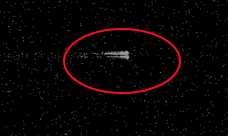
\includegraphics[width=0.4\linewidth]{fig6_CR/fig6A_CR.png}\label{fig:CR:A}}\\

\subfloat[B]{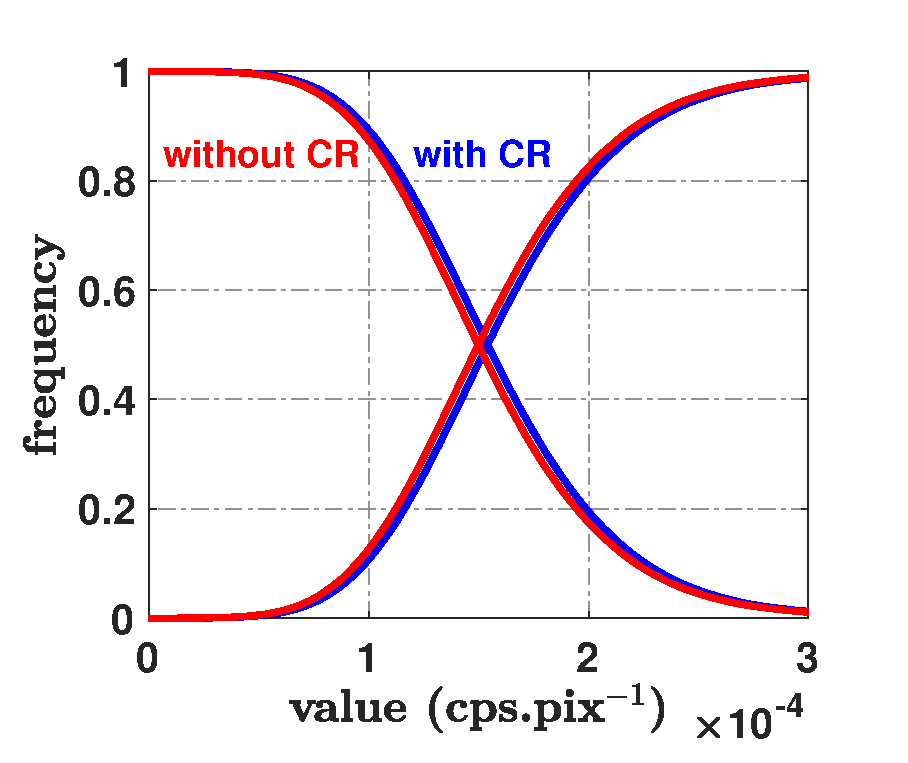
\includegraphics[width=0.4\linewidth]{fig6_CR/fig6B_CRCDF.eps}\label{fig:CR:B}} \qquad
\subfloat[C]{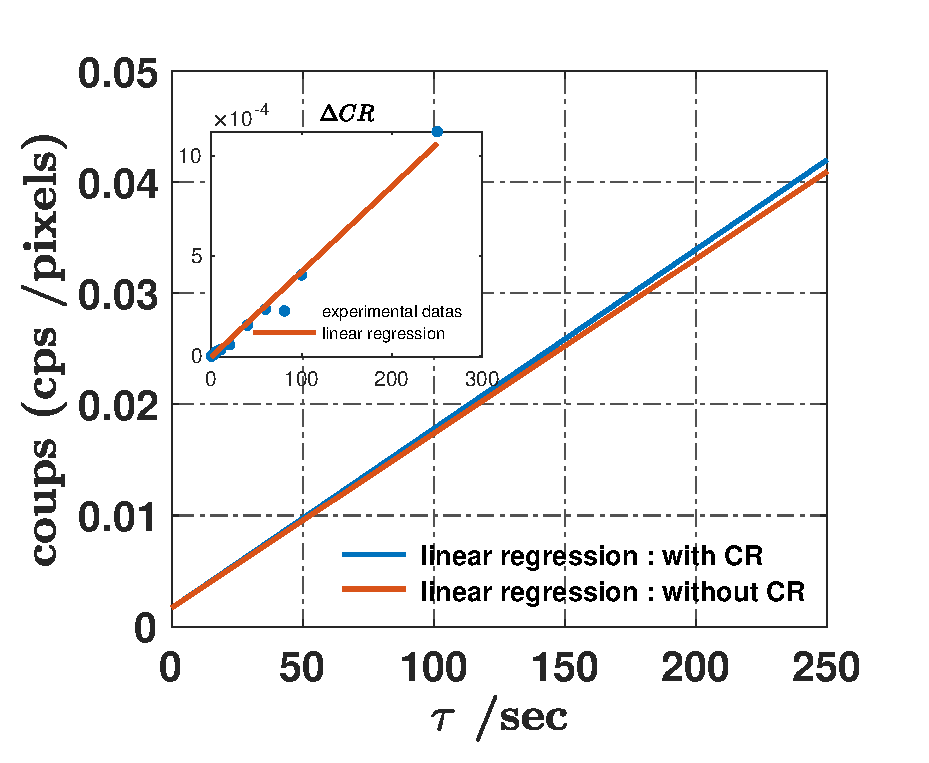
\includegraphics[width=0.4\linewidth]{fig6_CR/fig6C_CRfit.eps}\label{fig:CR:C}}


\caption{{\bf Cosmic Rays Frequency}. Aspect of a CR in a frame \subref{fig:CR:A}. The cumulative distributive function (CDF) and its complement of the frequency of counts \subref{fig:CR:B}, and the linear regression of the number of counts as a function of time is shown before and after removal of cosmic rays (CR) \subref{C}.  The experimental difference of the number of counts as a function of time before and after the removal of CR and its linear regression is on the insert of the figure \subref{fig:CR:C}.  }
\label{fig:CR}
\end{center}
\end{figure}

%%%%%%%%%%